% *********************************************************************
% © 2010–2021 Jeremy Sylvestre
%
% Permission is granted to copy, distribute and/or modify this document
% under the terms of the GNU Free Documentation License, Version 1.3 or
% any later version published by the Free Software Foundation; with no
% Invariant Sections, no Front-Cover Texts, and no Back-Cover Texts. A
% copy of the license is included in the appendix entitled “GNU Free
% Documentation License” that appears in the output document of this
% PreTeXt source code. All trademarks™ are the registered® marks of
% their respective owners.
%
% *********************************************************************

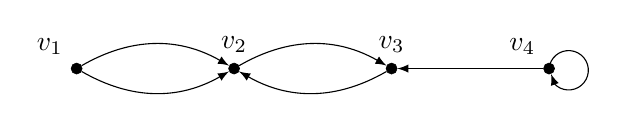
\begin{tikzpicture}[
	vertex/.style={ circle, draw, very thin, fill, inner sep=0pt, minimum size=4pt },
	vertexg/.style={ black!40!white, circle, draw, very thin, fill, inner sep=0pt, minimum size=4pt },
	vertexo/.style={ circle, draw, very thin, inner sep=0pt, minimum size=4pt }
]

\node at (-2,0) (v1) [vertex,label=above left:{$v_1$}] {};
\node at (0,0) (v2) [vertex,label=above:{$v_2$}] {};
\node at (2,0) (v3) [vertex,label=above:{$v_3$}] {};
\node at (4,0) (v4) [vertex,label=above left:{$v_4$}] {};
\draw[-latex] (v4) to (v3);
\draw[-latex] (v1) to [out=-30,in=-150] (v2);
\draw[-latex] (v1) to [out=30,in=150] (v2);
\draw[-latex] (v2) to [out=30,in=150] (v3);
\draw[-latex] (v3) to [out=210,in=-30] (v2);
\draw[-latex] (v4) arc (175:-135:0.25cm) -- (v4);

\end{tikzpicture}
